\renewcommand{\vec}[1]{\mathbf{#1}}
 \begin{enumerate}


\item First we need to show that $\vec{M}$ and $\vec{N}$ are the midpoints of $\vec{AB}$ and $\vec{CD}$ respectively.
%Take a circle C of radius $\vec{r}$=2cm, whose center is $\vec{O}$ such that $ \vec{O}$= $\begin{pmatrix}0\\0\end{pmatrix}$. 
In the given circle of center $\vec{O}$, let $\vec{AB}$ be an arbitrary chord such that $\vec{OX} \perp \vec{AB}$. We need to show that $\vec{AX}$ = $\vec{BX}$.
Since $\vec{OX} \perp \vec{AB}$ :\\
%(O-X).T(A-X)=0
$\begin{pmatrix}\vec{O-X}\end{pmatrix}^\vec{T}\begin{pmatrix}\vec{A-X}\end{pmatrix}$ = 0\\
$\implies \begin{pmatrix}\vec{-X[0]} & \vec{-X[1]}\end{pmatrix}\begin{pmatrix}\vec{A[0]-X[0]}\\\vec{A[1]-X[1]}\end{pmatrix}$ = 0\\ 
This condition is satisfied only when $ \vec{X}$ = $\frac{\vec{A+B}}{2}$\quad i.e.  $\vec{X}$ must be the midpoint of $\vec{AB}$.
\begin{comment}
\begin{enumerate}
	\item $\triangle OAX \cong \triangle OBX $by RHS rule as: 
	\begin{enumerate}
	\item $\angle{OXA} = \angle{OXB} $ \quad \{90\degree\}
	\item $\vec{OA} = \vec{OB}$ \quad \{radius of the circle\}
	\item $\vec{OX} = \vec{OX}$ \quad \{Common\}
	\end{enumerate}
\end{enumerate}
\end{comment}
\begin{equation}
	\therefore \vec{AX} = \vec{BX} \label{eq:1}
\end{equation}
Hence Perpendicular from the center of a circle to a chord bisects the chord.
  
\begin{figure}[!ht]
\centering
\resizebox{\columnwidth}{!}{
\begin{tikzpicture}
[scale=2,>=stealth,point/.style={draw,circle,fill = black,inner sep=0.5pt},]

%Triangle sides
\def\a{5}
\def\b{6}
\def\r{2}
%Coordinates of A
\def\p{1.414}
\def\q{-1.414}
\draw (0,0) circle (2cm);
%Labeling points
\node (A) at (\p,\q)[point,label=below right:$A$] {};
\node (B) at (\p, \p)[point,label=above right:$B$] {};
\node (X) at (\p, 0)[point,label=right:$X$] {};
\node (O) at (0,0)[point,label=left:$O$]{};
%Foot of median

%\node (D) at ($(A)!0.5!(O)$)[point,label=below:$D$] {};
%\node (E) at ($(A)!0.5!(B)$)[point,label=left:$E$] {};
%\node (F) at ($(C)!0.5!(A)$)[point,label=right:$F$] {};

%Drawing triangle ABC
\draw (A) --  (B) -- node[above] {$\textrm{r}$} (O) -- node[below] {$\textrm{r}$} (A);
\draw (X)-- (O);
%Drawing medians BE and CF
%\draw (D) -- (E);
%\draw (D) -- (F);
%\draw (O) -- (B);
%\draw (O) -- (C);
%Drawing EF
%\draw (E) -- (F);

%Labeling sides
%\node [right] at ($(A)!0.5!(E)$) {$\frac{b}{2}$};
%\node [right] at ($(C)!0.5!(E)$) {$\frac{b}{2}$};
%\node [left] at ($(B)!0.5!(F)$) {$\frac{c}{2}$};
%\node [left] at ($(A)!0.5!(F)$) {$\frac{c}{2}$};

%Angles
\tkzMarkRightAngle[fill=green!60,size=.27](O,X,B)
\tkzMarkRightAngle[fill=yellow!60,size=.27](O,X,A)
%\tkzMarkAngle[fill=green!60,size=.3](O,B,A)
%
%\tkzMarkAngle[fill=red!60,size=.7](A,F,D)
%\tkzMarkAngle[fill=red!60,size=.7](A,C,O)
%%
%\tkzMarkAngle[fill=yellow!60,size=.2](A,D,E)
%\tkzMarkAngle[fill=yellow!60,size=.2](A,O,B)
%%
%\tkzMarkAngle[fill=orange!60,size=.2](F,D,A)
%\tkzMarkAngle[fill=orange!60,size=.2](C,O,A)
%
%\tkzMarkAngle[fill=blue!60,size=.3](E,A,F)
\end{tikzpicture}
}
\caption{Perpendicular from the center of a circle to a chord bisects the chord}
\label{fig:steponetex}	
\end{figure}




\item Next we need to show that equal chords of a circle are equidistant from the center.\\

In the circle given in Fig:\ref{fig:steptwotex} whose center is $\vec{O}$, let $\vec{AB}$ and $\vec{CD}$ be two arbitrary chords such that $\vec{OX} \perp \vec{AB}$ and $\vec{OY} \perp \vec{CD}$. We need to show that $\vec{OX}$ = $\vec{OY}$.
%\newline
 

\begin{enumerate}
	
	\item Since $\vec{OX} \perp \vec{AB}$, $\vec{AX} =  \vec{BX} = \frac{\vec{AB}}{2}$ \{From:\eqref{eq:1} \}\\
	Similarly $\vec{CY} =  \vec{DY} = \frac{\vec{CY}}{2}$\\
	\item As $\vec{AB} =  \vec{CD}$\\
	$\frac{\vec{AB}}{2} = \frac{\vec{CD}}{2}$\\
	Hence 
	\begin{equation}
	\vec{AX} =  \vec{CY} \label{eq:2}
	\end{equation}
	
	\item In $\triangle AOX$ and $\triangle COY $ as shown in Fig.\ref{fig:steptwotex} using baudhayana theorem
	\begin{equation}
	\| \vec{O-Y}\|^2 + \|\vec{Y-C}\|^2 = \|\vec{O-X}\|^2 + \|\vec{X-A}\|^2
	\end{equation}
	Using \eqref{eq:2}, $\| \vec{O-Y}\|^2 = \|\vec{O-X}\|^2$\\
$	\implies \| \vec{O-Y}\| = \| \vec{O-X}\|$
\begin{comment}	
	\begin{enumerate}
	\item $\angle{OXA} = \angle{OYC} $ \quad \{90\degree\}
	\item $\vec{OA} = \vec{OC}$ \quad \{radius of the circle\}
	\item $\vec{AX} = \vec{CY}$ \quad \{From:\eqref{eq:2}\}
	\end{enumerate}
	Hence  $\triangle AOX \cong \triangle COY $ by RHS rule.\\
\end{comment}
	
	\begin{equation}
	Therefore, \vec{OX}=\vec{OY} \label{eq:3}
	\end{equation}
\end{enumerate}
	Hence the equal chords of a circle are equidistant from the center.\\

  
\begin{figure}[!ht]
\centering
\resizebox{\columnwidth}{!}{
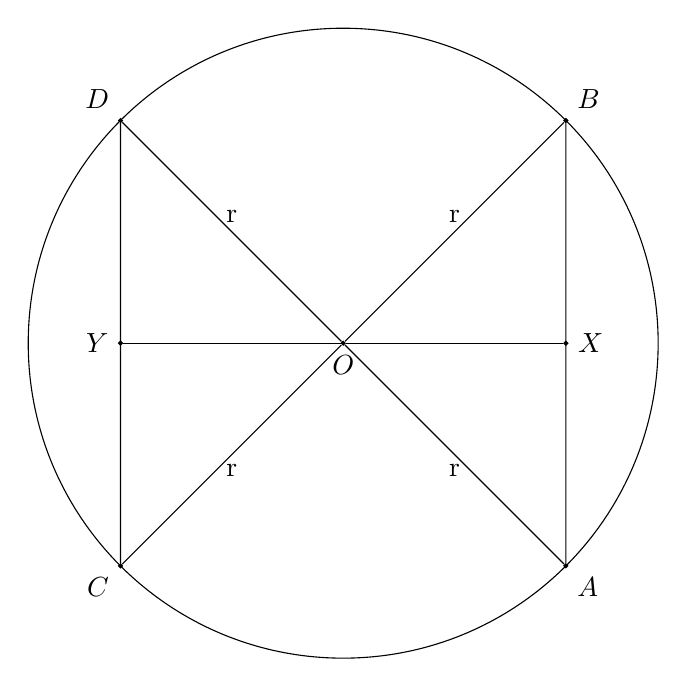
\begin{tikzpicture}
[scale=2,>=stealth,point/.style={draw,circle,fill = black,inner sep=0.5pt},]

%Triangle sides
\def\a{5}
\def\b{6}
\def\r{2}
%Coordinates of A
\def\p{1.414}
\def\q{-1.414}
\draw (0,0) circle (2cm);
%Labeling points
\node (A) at (\p,\q)[point,label=below right:$A$] {};
\node (B) at (\p, \p)[point,label=above right:$B$] {};
\node (X) at (\p, 0)[point,label=right:$X$] {};

\node (C) at (\q,\q)[point,label=below left:$C$] {};
\node (D) at (\q, \p)[point,label=above left:$D$] {};
\node (Y) at (\q, 0)[point,label=left:$Y$] {};

\node (O) at (0,0)[point,label=below:$O$]{};

%Drawing triangle ABC
\draw (A) --  (B) -- node[above] {$\textrm{r}$} (O) -- node[below] {$\textrm{r}$} (A);
\draw (X)-- (O);
\draw (C) --  (D) -- node[above] {$\textrm{r}$} (O) -- node[below] {$\textrm{r}$} (C);
\draw (Y)-- (O);
%Drawing medians BE and CF
%\draw (D) -- (E);
%\draw (D) -- (F);
%\draw (O) -- (B);
%\draw (O) -- (C);
%Drawing EF
%\draw (E) -- (F);

%Labeling sides
%\node [right] at ($(A)!0.5!(E)$) {$\frac{b}{2}$};
%\node [right] at ($(C)!0.5!(E)$) {$\frac{b}{2}$};
%\node [left] at ($(B)!0.5!(F)$) {$\frac{c}{2}$};
%\node [left] at ($(A)!0.5!(F)$) {$\frac{c}{2}$};

%Angles
\tkzMarkRightAngle[fill=green!60,size=.27](O,X,A)
\tkzMarkRightAngle[fill=orange!60,size=.27](O,Y,C)
%\tkzMarkAngle[fill=green!60,size=.3](O,B,A)
%
%\tkzMarkAngle[fill=red!60,size=.7](A,F,D)
%\tkzMarkAngle[fill=red!60,size=.7](A,C,O)
%%
%\tkzMarkAngle[fill=yellow!60,size=.2](A,D,E)
%\tkzMarkAngle[fill=yellow!60,size=.2](A,O,B)
%%
%\tkzMarkAngle[fill=orange!60,size=.2](F,D,A)
%\tkzMarkAngle[fill=orange!60,size=.2](C,O,A)
%
%\tkzMarkAngle[fill=blue!60,size=.3](E,A,F)
\end{tikzpicture}
}
\caption{Equal chords of a circle are equidistant from the center}
\label{fig:steptwotex}	
\end{figure}


The  following Python code generates Fig. \ref{fig:stepthree}\\
    \begin{lstlisting}
        ./codes/step3.py
    \end{lstlisting}

    \begin{figure}[!ht]
	\centering
	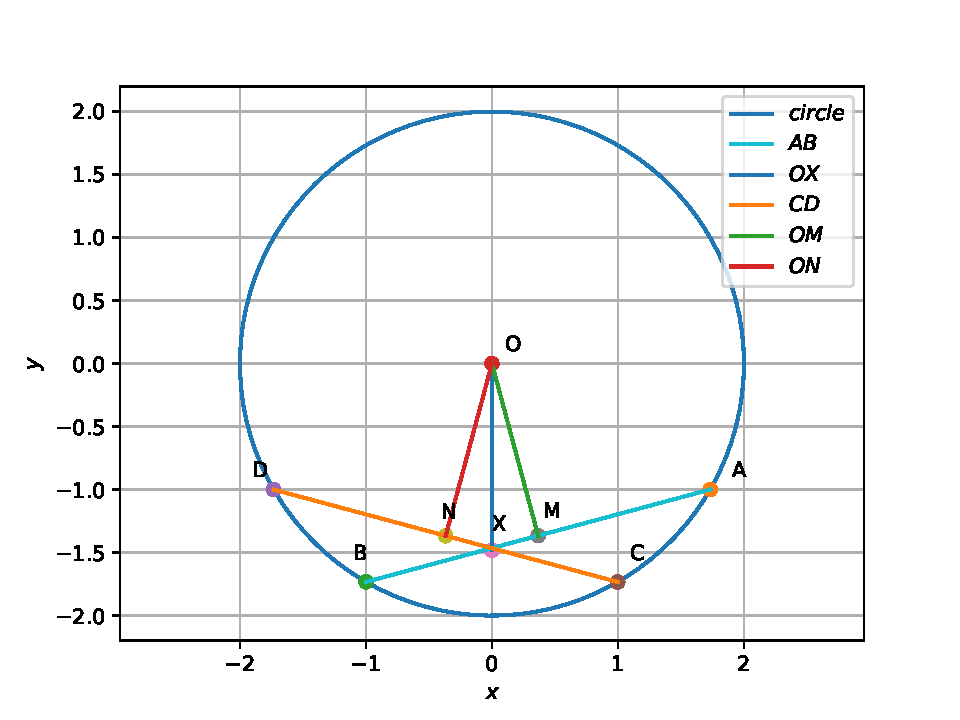
\includegraphics[width=\columnwidth]{./figs/step3.pdf}
	\caption{Circle generated using python}
	\label{fig:stepthree}
    \end{figure}
      The equivalent \LaTeX{}- tikz code generating Fig. \ref{fig:stepthreetex} is
    \begin{lstlisting}
        ./figs/stepthree.tex
    \end{lstlisting}
	
	The above \LaTeX{} code can be compiled as a standalone document as
	\begin{lstlisting}
	./figs/step3_standalone.tex
	\end{lstlisting}


\item In the circle given in Fig.\ref{fig:stepthreetex} we need to show that $\angle{OXA}$ = $\angle{OXD}$. We draw $\vec{OM} \perp \vec{AB}$ and $\vec{ON} \perp \vec{CD}$.\\
In $\triangle OMX$ and $\triangle ONX$,using baudhayana theorem
	\begin{equation}
	\| \vec{N-O}\|^2 + \|\vec{X-N}\|^2 = \|\vec{M-O}\|^2 + \|\vec{X-M}\|^2
	\end{equation}
	Using \eqref{eq:3}, $\| \vec{X-N}\|^2 = \|\vec{X-M}\|^2$\\
\begin{equation}
	\implies \| \vec{NX}\| = \| \vec{MX}\| \label{eq:4}
\end{equation}
In $\triangle OMX$ and $\triangle ONX$,using cosine formula\\
\begin{equation}
\cos{\angle{OXN}} = \frac{  \|\vec{NX}\|^2 + \|\vec{OX}\|^2  - \|\vec{ON}\|^2     }{2\|\vec{NX}\|\|\vec{OX}\|}
\end{equation}
\begin{equation}
\cos{\angle{OXM}} = \frac{  \|\vec{MX}\|^2 + \|\vec{OX}\|^2  - \|\vec{OM}\|^2     }{2\|\vec{MX}\|\|\vec{OX}\|}
\end{equation}
Using \eqref{eq:4} and \eqref{eq:3} 
\begin{equation}
\cos{\angle{OXN}} = \cos{\angle{OXM}}
\end{equation}

\begin{comment}
\begin{enumerate}
	\item $\angle{OMX} = \angle{ONX} $ \quad \{90\degree\}
	\item $\vec{OM} = \vec{ON}$ \quad \{From:\eqref{eq:3}\}
	\item $\vec{OX} = \vec{OX}$ \quad \{Common\}
\end{enumerate}
Hence  $\triangle OMX \cong \triangle ONX $ by RHS rule.\\
\end{comment}
	Therefore, $\angle{OXM} = \angle{OXN}$\\
$	\implies \angle{OXA} = \angle{OXD}$\\

Hence Proved.





\end{enumerate}




